\section{Implementierung}
\label{sec:Implementierung}

Ziel dieses Kapitels ist die detaillierte Darstellung der technischen Umsetzung des entwickelten Retrieval-Augmented-Generation-(RAG)-Systems. Der Fokus liegt auf der Verarbeitung der Dokumente, der hybriden Suchstrategie sowie der Realisierung der einzelnen Systemkomponenten.

Das System verfolgt das Ziel, nutzerspezifische Anfragen im Kontext von Vergabedokumenten präzise und kontextbasierte Antworten zu erzeugen. Hierzu werden relevante Dokumentinhalte identifiziert, aufbereitet und als Grundlage für die Generierung der Antworten verwendet.

\subsection{Datenaufbereitung und Chunking}

Die Grundlage des Systems bilden Dokumente im PDF-Format, deren Inhalte zunächst extrahiert und anschließend in kleinere Textsegmente (Chunks) unterteilt werden. Dieser Schritt ist erforderlich, um eine effiziente Indexierung sowie eine präzise semantische Suche zu ermöglichen.

Die Zerlegung erfolgt anhand einer festen Chunk-Größe mit zusätzlicher Überlappung. Die Überlappung stellt sicher, dass relevante Informationen an Segmentgrenzen nicht verloren gehen und der semantische Zusammenhang erhalten bleibt.

Die Wahl der Chunk-Größe stellt einen Kompromiss zwischen Kontexttiefe und Retrieval-Effizienz dar. Während zu große Segmente zu unscharfen Treffern führen können, besteht bei zu kleinen Segmenten die Gefahr eines Verlusts semantischer Zusammenhänge.

\begin{lstlisting}[language=Python, caption={Chunking-Verfahren}, label={lst:chunking}]
def chunk_text(text: str, chunk_size: int = CHUNK_SIZE, overlap: int = CHUNK_OVERLAP):
    chunks = []
    for i in range(0, len(text), chunk_size - overlap):
        chunk = text[i:i + chunk_size]
        if chunk.strip():
            chunks.append(chunk)
    return chunks
\end{lstlisting}

Die Extraktion der Inhalte erfolgt seitenweise aus den PDF-Dokumenten:

\begin{lstlisting}[language=Python, caption={PDF-Text-Extraktion}, label={lst:pdf}]
reader = PdfReader(io.BytesIO(content_bytes))
for page in reader.pages:
    text += page.extract_text() or ""
\end{lstlisting}

Die erzeugten Textsegmente bilden die Grundlage für die nachfolgende Indexierung sowie die spätere Informationssuche.

\begin{figure}[h!]
\centering

\includegraphics[width=1\textwidth]{Chunking.png}
\caption{Verarbeitung von PDF-Dokumenten zu Text-Chunks}
\label{fig:chunking}
\end{figure}

\subsection{Hybride Suche}

Die Informationssuche basiert auf einer hybriden Strategie, die klassische lexikalische Suche (BM25) mit semantischer Vektorsuche kombiniert. Während BM25 insbesondere exakte Wortübereinstimmungen berücksichtigt, ermöglicht die Vektorsuche das Auffinden semantisch ähnlicher Inhalte.

Zur Reduktion der Latenz werden beide Suchverfahren parallel ausgeführt:

\begin{lstlisting}[language=Python, caption={Parallele Hybrid-Suche}, label={lst:hybrid}]
def search_hybrid(query: str, intent: str):
    with ThreadPoolExecutor(max_workers=2) as pool:
        future_bm25 = pool.submit(search_bm25, query, intent, 15)
        future_emb = pool.submit(get_embedding, query)

query_embedding = future_emb.result()
bm25_hits = future_bm25.result()

vector_hits = search_vector(query_embedding, size=15)

final_hits, max_score = reciprocal_rank_fusion(bm25_hits, vector_hits)
return final_hits, max_score

\end{lstlisting}

Die Zusammenführung der Ergebnisse erfolgt mittels Reciprocal Rank Fusion (RRF). Dieses Verfahren kombiniert die Ranglisten beider Suchmethoden und ermöglicht eine robuste, skalierungsunabhängige Bewertung der Gesamtrelevanz.

\begin{figure}[h!]
\centering
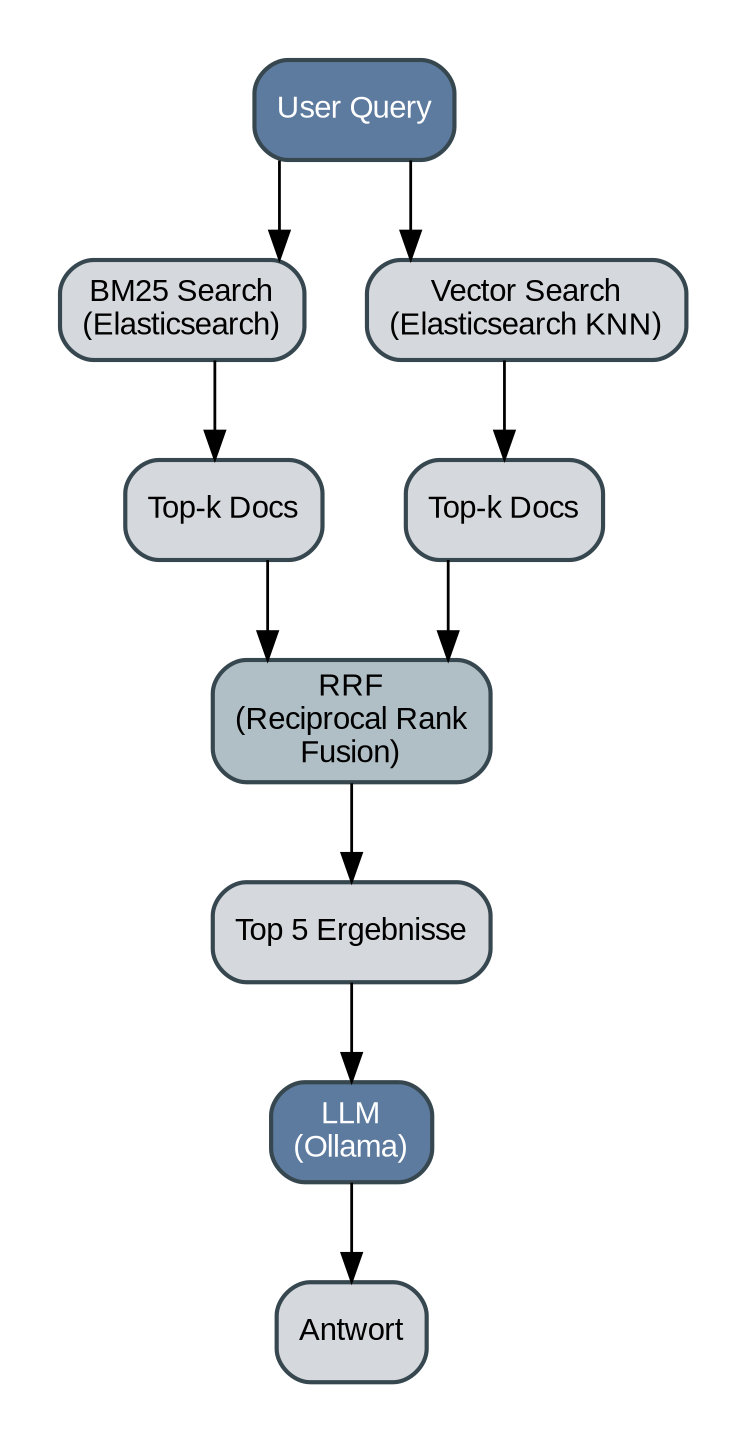
\includegraphics[width=0.8\textwidth]{Hybrid_Search.png}
\caption{Ablauf der hybriden Suche mit BM25, Vektorsuche und RRF}
\label{fig:hybrid}
\end{figure}

\clearpage

\subsection{Backend-Architektur mit FastAPI}

Das Backend wurde mit dem Framework FastAPI realisiert und fungiert als zentrale Orchestrierungsschicht des Systems. Es übernimmt die Verarbeitung eingehender Anfragen und koordiniert die Kommunikation zwischen den einzelnen Komponenten.

Dabei verbindet das Backend die Retrieval-Komponente (Elasticsearch), das Sprachmodell (über Ollama) sowie das Frontend.

\begin{lstlisting}[language=Python, caption={FastAPI Initialisierung}, label={lst:fastapi}]
app = FastAPI(
    title="RAG API - Bachelor Arbeit",
    version="1.0.0"
)

app.include_router(query_router, prefix="/api")
\end{lstlisting}

Zur Überprüfung der Systemverfügbarkeit wurde ein Health-Endpunkt implementiert:

\begin{lstlisting}[language=Python, caption={Health Endpoint}, label={lst:health}]
@app.get("/health")
async def health():
    return {"status": "healthy"}
\end{lstlisting}

Der Endpunkt \texttt{/api/ask} stellt die zentrale Schnittstelle dar und bildet den vollständigen RAG-Prozess ab.

\begin{figure}[h!]
\centering
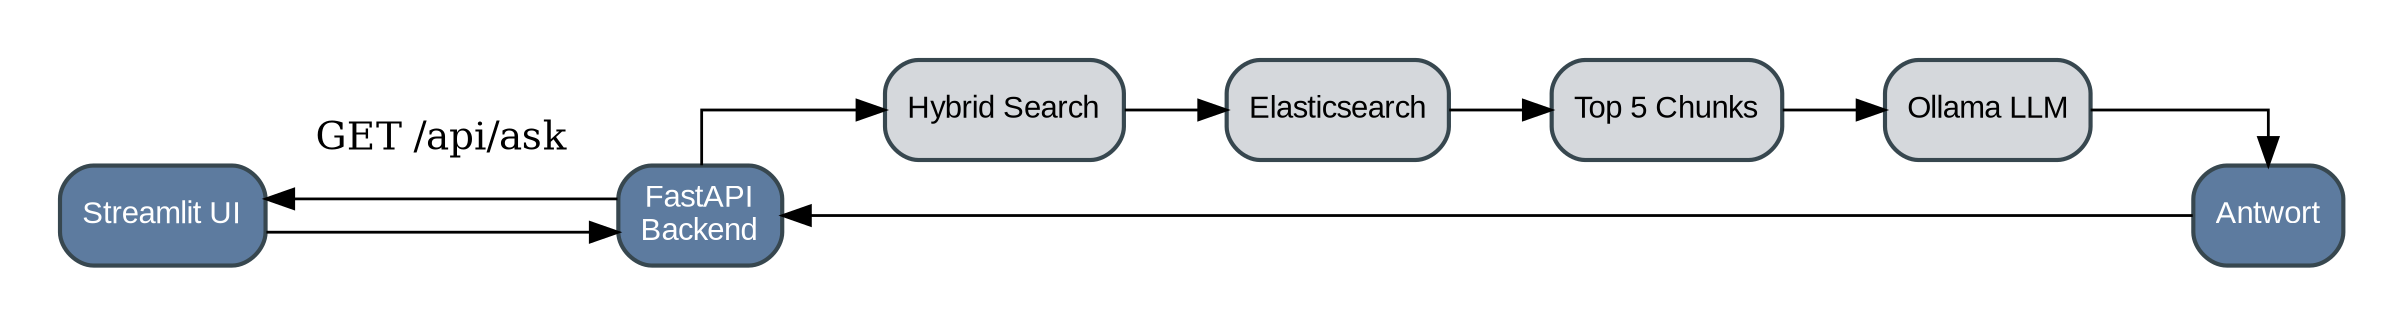
\includegraphics[width=1\textwidth]{API_Flow.png}
\caption{Ablauf einer Anfrage durch das Backend}
\label{fig:backend}
\end{figure}

\subsection{LLM-Integration und Prompting}

Die Generierung der Antworten erfolgt durch ein lokal betriebenes Large Language Model über die Ollama-Schnittstelle. Das Modell erhält sowohl die Nutzeranfrage als auch den zuvor ermittelten Kontext als Eingabe.

Das Sprachmodell verfügt über keinen direkten Zugriff auf externe Wissensquellen, sondern basiert ausschließlich auf dem bereitgestellten Kontext (Closed-Book-Ansatz).

Der Prompt wird dynamisch aufgebaut, um sicherzustellen, dass die Antwort ausschließlich auf den bereitgestellten Informationen basiert:

\begin{lstlisting}[language=Python, caption={Prompt-Erstellung}, label={lst:prompt}]
def build_prompt(query: str, context: str, intent: str, model: str) -> str:
    return f"""
KONTEXT:
{context}

FRAGE: {query}

Basiere deine Antwort nur auf dem Kontext.
"""
\end{lstlisting}

Diese Struktur trägt maßgeblich zur Reduktion von Halluzinationen bei und erhöht die Nachvollziehbarkeit der generierten Antworten.

\subsection{Antwortvalidierung}

Zur weiteren Verbesserung der Antwortqualität wurde ein zusätzlicher Validierungsschritt implementiert. Dabei wird überprüft, ob die generierte Antwort durch den bereitgestellten Kontext gestützt ist.

Die Validierung erfolgt durch eine modellbasierte Klassifikation der Antwort hinsichtlich ihrer Übereinstimmung mit dem Kontext.

\begin{lstlisting}[language=Python, caption={Faithfulness Check}, label={lst:faithfulness}]
def check_faithfulness(query: str, context: str, answer: str, model: str):
    if "JA" in verdict:
        return answer
    return FALLBACK_ANSWER
\end{lstlisting}

Falls die Antwort nicht ausreichend gestützt ist, wird eine alternative Antwort ausgegeben. Dieser Mechanismus reduziert das Risiko halluzinierter Inhalte.

\subsection{Frontend-Implementierung mit Streamlit}

Für die Benutzerinteraktion wurde ein webbasiertes Frontend mit Streamlit realisiert. Dieses ermöglicht die Eingabe natürlichsprachlicher Anfragen sowie die Darstellung der generierten Antworten in Form eines Chat-Interfaces.

Das Frontend dient ausschließlich der Interaktion und enthält keine Geschäftslogik, wodurch eine klare Trennung zwischen Präsentations- und Verarbeitungsschicht gewährleistet wird.

\begin{lstlisting}[language=Python, caption={Chat-Eingabe im Frontend}, label={lst:frontend}]
user_query = st.chat_input("Stellen Sie Ihre Frage")

if user_query:
    data = call_ask_api(user_query, selected_model)
\end{lstlisting}

\begin{figure}[h!]
\centering
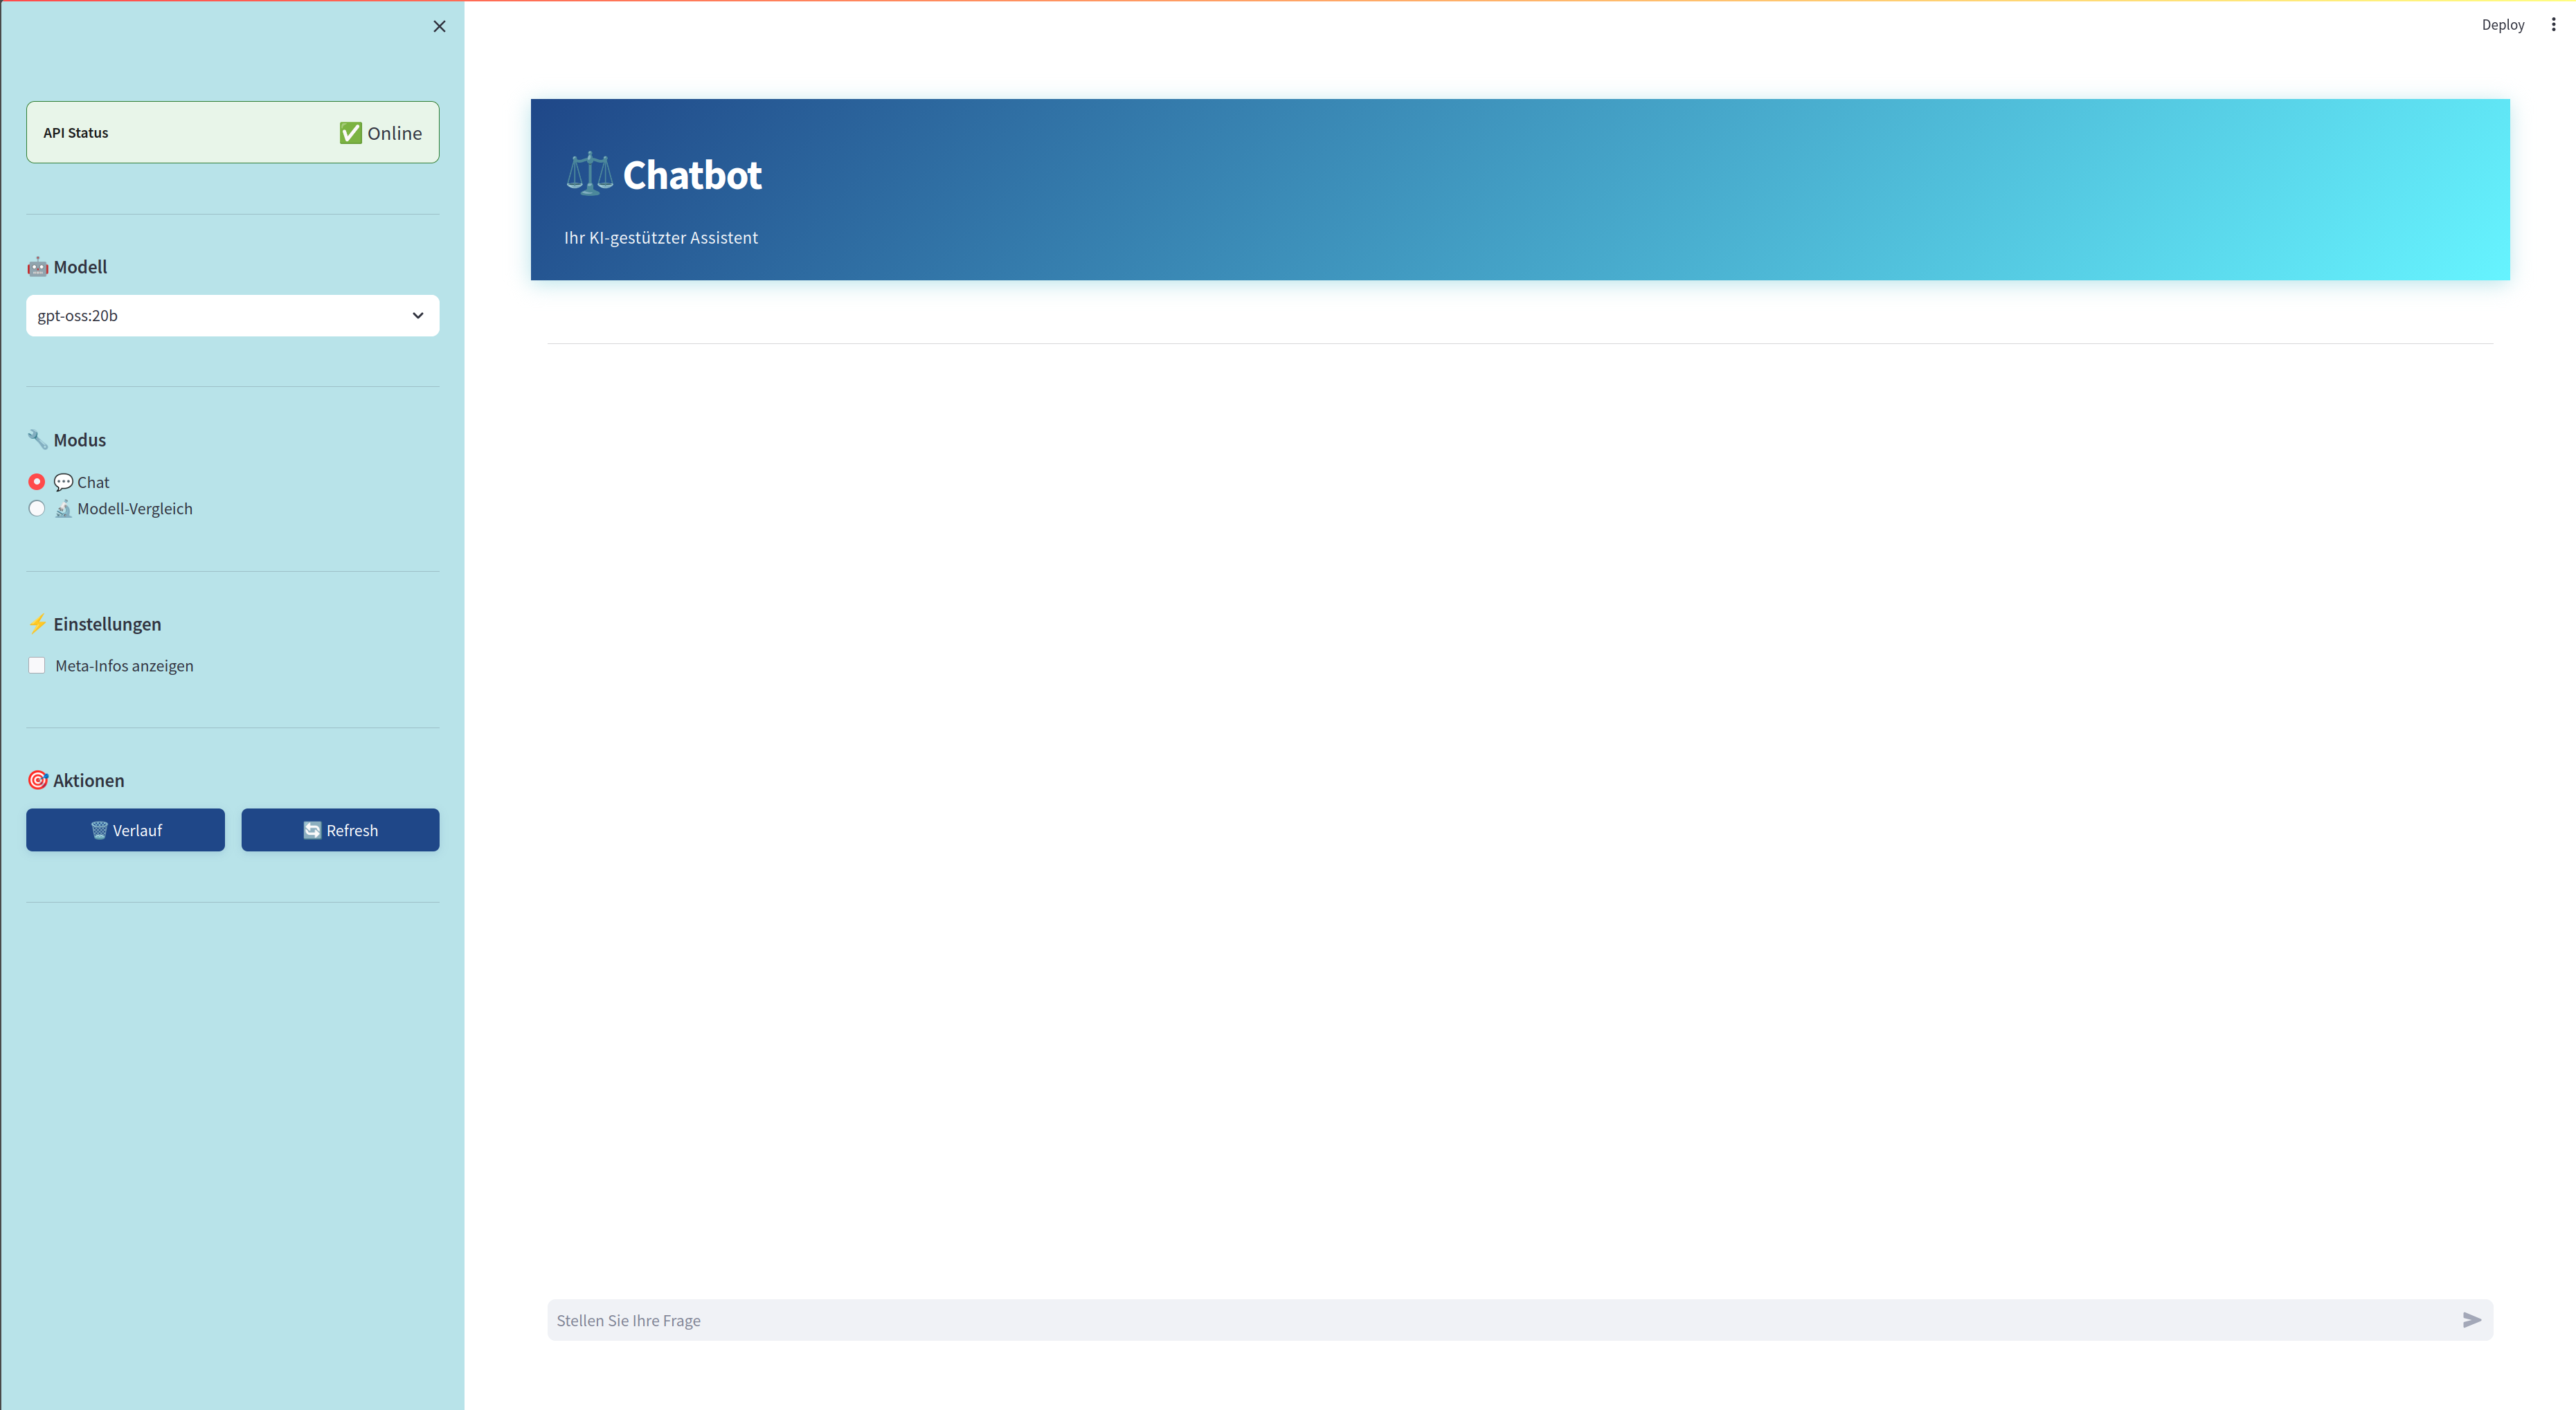
\includegraphics[width=0.9\textwidth]{frontend.png}
\caption{Benutzeroberfläche des Systems}
\label{fig:frontend}
\end{figure}

\subsection{Konfiguration}

Zentrale Systemparameter werden in einer Konfigurationsdatei definiert, um eine flexible Anpassung des Systems zu ermöglichen:

\begin{lstlisting}[language=Python, caption={Systemparameter}, label={lst:config}]
CHUNK_SIZE = 1000
HYBRID_BM25_W = 0.4
HYBRID_VECTOR_W = 0.6
\end{lstlisting}

Diese Parameter beeinflussen maßgeblich die Qualität der Suche sowie die Performance des Systems.

\subsection{Zusammenfassung}

Die Implementierung integriert Datenaufbereitung, hybride Suche, Backend-Architektur, Sprachmodellintegration sowie ein interaktives Frontend zu einem leistungsfähigen Gesamtsystem.

Die gewählte Architektur stellt einen Kompromiss zwischen Antwortqualität, Systemlatenz und Komplexität dar. Insbesondere die Kombination aus hybrider Suche und nachgelagerter Validierung trägt wesentlich zur Verbesserung der Ergebnisqualität bei und ermöglicht eine robuste, nachvollziehbare Verarbeitung natürlichsprachlicher Anfragen im Vergabekontext.

\clearpage